\section[Studentische Mitbestimmung]{Studentische Mitbestimmung~I\\Die verfasste Studierendenschaft}
\label{studmit}
\begin{multicols*}{2}
Die verfasste Studierendenschaft ist, wie der Name es schon andeutet, durch die Verfassung gesetzlich an jeder Universität vorgeschrieben.
Diese ist als eine Selbstorganisation von Studierenden zu verstehen, in Serviceleistungen sowie in politischen Fragestellungen.
Sie wird auf unterschiedlichen Wegen von der Studierendenschaft gewählt.
So findet einmal im Jahr im Sommersemester eine wichtige Wahl zum Studierendenparlament und den Fachschaftsvertretungen statt.
Außerdem besteht der AStA auch noch aus den unpolitischen, autonomen Referaten, welche auch von Teilgruppen (sogenannte Statusgruppen) der Studierendenschaft gewählt werden.

\bigskip
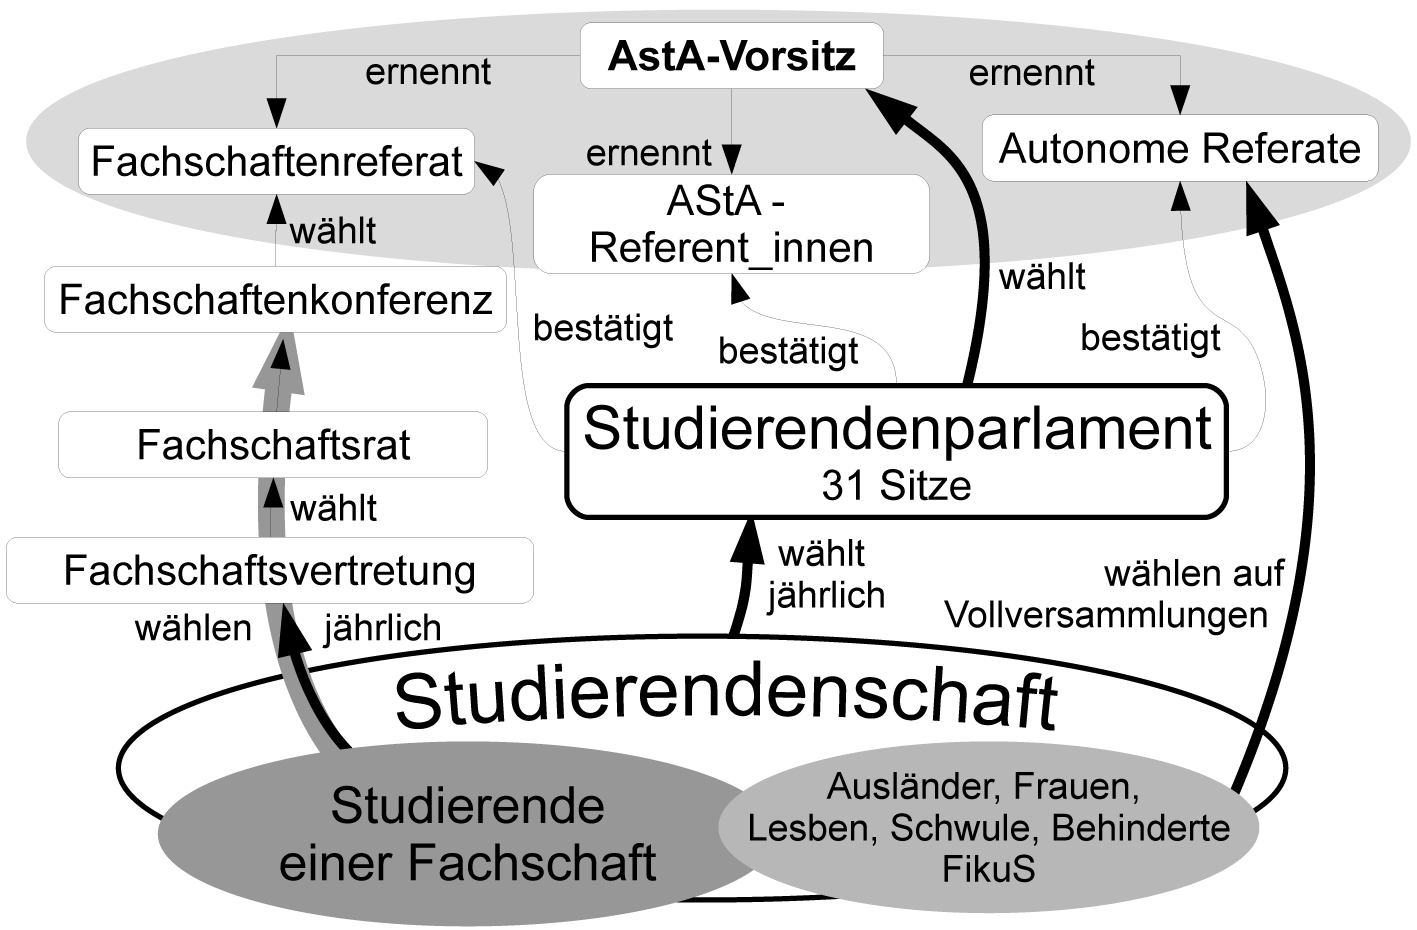
\includegraphics[width=\columnwidth]{res/verfasste_studierendenschaft.png}
\bigskip

\subsection{Das Studierendenparlament}
Das StuPa wird Ende Juni gewählt und ist  in seiner Rolle – nun ja – das Parlament der Studierendenschaft. Es wird in Verhältniswahl jährlich neu gewählt, wobei Listen antreten, die meist Parteien nahe stehen. Entsprechend bilden sich Fraktionen mit unterschiedlichen politischen Ansichten heraus.
Hier wird der AStA ("die Regierung") gewählt – normalerweise durch Koalitionen, in denen Fraktionen welche gemeinsam eine Mehrheit haben gemeinsam einen AStA bilden. Das StuPa bestätigt die Referate des AStA und hat finanzielle Kontrolle über diesen, d.h. Haushalt und Anschaffungen des AStA müssen vom StuPa bestätigt werden. Desweiteren wird auf die Nöte und Interessen der Studierendenschaft aufmerksam gemacht (z.\,B. durch Resolutionen) und es werden studentische Initiativen unterstützt

\subsection{Der AStA}
Der Allgemeine Studierenden-Ausschuss ist so etwas wie die Regierung der Studierendenschaft.
Hier wird die politische Richtung vorgegeben und der AStA-Vorsitz darf die Beiträge, die die Studierenden semesterweise bezahlen, verwalten.
Neben Vortragsreihen und kleineren Aktionen werden hiervon insbesondere solidarisch für alle das Semesterticket und die Serviceangebote (siehe Kasten rechts) des AStA finanziert. Zum AStA gehören eine Reihe an Referaten, die dessen Verwaltungsaufgaben wahrnehmen und Autonome Referate, welche die Interessen verschiedener Teilgruppen der Studierendenschaft vertreten und z.\,B. Angebote genau für diese organisieren.

\subsection{Die Fachschaftsräte}
Die Fachschaftsvertretungen~(FSV) werden jährlich zusammen mit dem StuPa gewählt.
Die Aufgabe einer FSV ist die Wahl und Kontrolle des jeweiligen Fachschaftsrats~(FSR), der die Tagesgeschäfte leitet.
Die FSV wird von allen Mitgliedern einer Fachschaft~(FS) gewählt.

Zur FS gehören in der Physik alle für einen Studiengang der Physik eingeschriebenen Studierenden, also wahrscheinlich auch der Leser dieses Heftes.
Das Wort Fachschaft steht allerdings auch umgangssprachlich für:
\begin{itemize}
	\item den Fachschaftsrat, welcher den Hauptteil der Gremienarbeit, d.h. die Vertretung studentischer Interessen in den Gremien des Fachbereichs, leistet und auch die O-Woche organisiert, das Sommerfest plant und Klausuren/Prüfungsprotokolle verleiht.
Dieser ist meistens gemeint, wenn jemand von "der Fachschaft" spricht.
	\item den Fachschaftsraum am Eingang der KP/TP, wo wir gerne die Studierenden beraten oder Klausuren verleihen.
\end{itemize}
\emph{Die Fachschaft Physik trifft sich jeden Mittwoch um 18~Uhr im Fachschaftsraum.
Die Sitzungen sind grundsätzlich öffentlich und neue Gesichter sind immer gerne gesehen!}

\subsection{Die Fachschaftenkonferenz}
In der FK treffen sich Vertreter der Fachschaftsräte jeden Dienstag um 18~Uhr, um sich untereinander auszutauschen.
Die FK wird von den autonomen AStA-Fachschaftenreferenten geleitet.
Diese unterstützen die Fachschaften auch bei der Koordinierung untereinander und informiert alle Fachschaften über aktuelle Änderungen in der Hochschulpolitik sowie über Veranstaltungen, die die einzelnen Fachschaften ausrichten.

\fibelsig{Friedrich, Justus}
\end{multicols*}

\clearpage

\section*{Studentische Mitbestimmung~II\\Die universitären Strukturen}
\begin{multicols*}{2}
\begin{quote}
	\textit{Wäre es da nicht doch einfacher, die Regierung löste das Volk auf und wählte ein anderes?}
	
	\hfill--- Bertold Brecht
\end{quote}
Die Universität selbst ist demokratisch aufgebaut , wobei die Gremien durch die Statusgruppen der Universität, die Studierenden, die Mitarbeiter und die Professoren nach festen Verhältnissen gebildet werden, wobei die Entsendung jeweils durch Wahl innerhalb der Statusgruppe geschieht.
Die Professoren haben in der Regel absolute Mehrheit. Seit einigen Jahren werden die wichtigsten Entscheidungen im Hochschulrat getroffen, welcher viele externe, durch das Kultusministerium eingesetzte Mitglieder beinhaltet und eine Ausnahme zur ansonsten demokratisch ablaufenden Verwaltung darstellt.

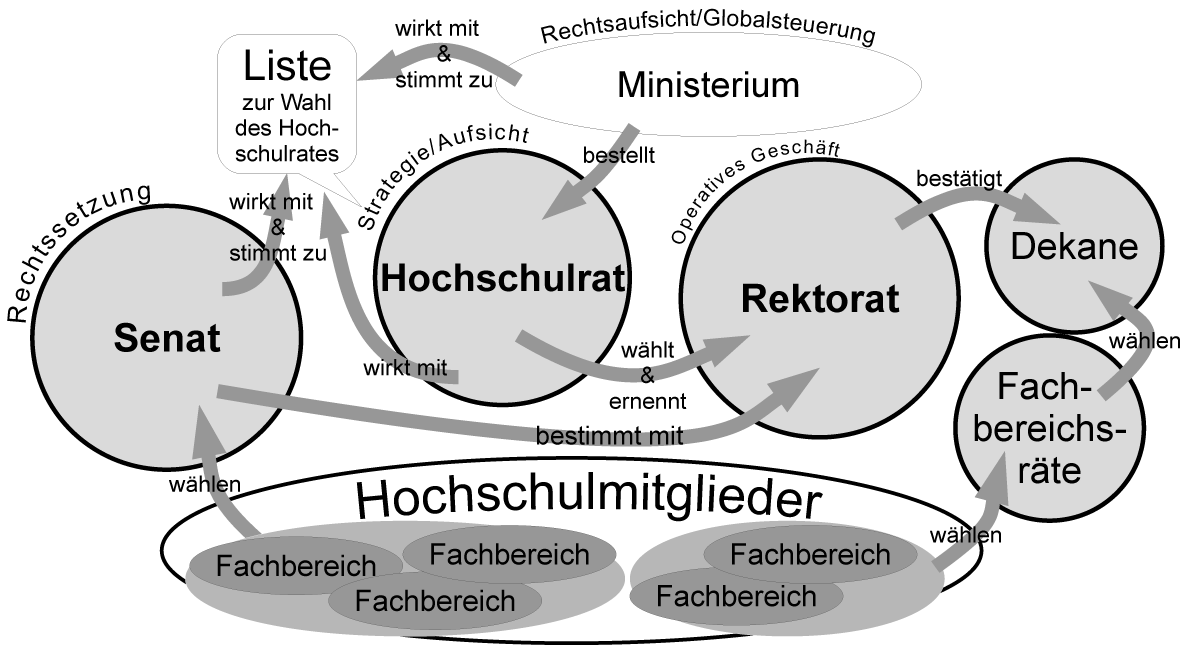
\includegraphics[width=\columnwidth]{res/uni_strukturen.png}

\subsection{Die Fachbereichsräte}
Der FBR ist an einem Fachbereich, also auch in der Physik, das wichtigste Gremium.
Hier wird über die wichtigen Entscheidungen des Dekanats abgestimmt sowie über Berufungen Kommissionen eingerichtet und der Studienbeirat eingesetzt, um die Prüfungsordnungen und deren stetige Verbesserung zu diskutieren.
Die studentischen FBR-Mitglieder (3 reguläre Mitglieder und 3 Stellvertreter) werden im Sommersemester zeitgleich mit den Wahlen der verfassten Studierendenschaft von den Studierenden am Fachbereich gewählt.
Sie stehen euch gerne mit Rat zur Verfügung; ihr könnt sie, wie auch die studentischen Mitglieder des Studienbeirats, über die Fachschaft erreichen, um auf Verbesserungen oder Missstände im Studium hinzuweisen.

\subsection{Der Senat}
Der Senat ist das wichtigste Gremium; hier werden Entscheidungen über Berufungen von Professoren, die Prüfungsordnungen der Fachbereiche und vieles weitere, was die gesamte Uni betrifft, getroffen.
So wird hier auch der Haushaltsplan von der eingesetzten Finanzkommission erstellt.
Weitere Kommissionen des Senats sind z.\,B.\ die Bibliothekskommission.
Die Senatswahl wird ebenfalls gemeinsam mit den anderen Wahlen abgehalten.

\begin{center}
	% Länge „\fboxsep“: Abstand zwischen Inhalt und Rahmen
	\setlength{\fboxsep}{2mm}
	\framebox[\columnwidth]{
	\begin{minipage}{0.95\columnwidth}
		\setlist[itemize]{label={}, nosep, topsep=\smallskipamount, itemsep=\smallskipamount, after={\smallskip}, leftmargin=1.5em}
		\begin{center}
			\large\textbf{Service des AStA}
		\end{center}
		
		\medskip
		
		Der AStA bietet folgende Serviceangebote an:
		
		\smallskip
		
		\textit{AStA-Büro:}
		\begin{itemize}
			\item Beglaubigte Kopien von Dokumenten
			\item Internationale Studierendenausweise
			\item Bulli-Verleih
			\item Semesterticket
			\item HiFi-Anlagen-Verleih
		\end{itemize}
		
		\textit{Beratungsstellen:}
		\begin{itemize}
			\item Rechtsberatung
			\item BAföG- und Sozialberatung
			\item Beschwerdestelle
		\end{itemize}
		
		\textit{Druckerei:}
		\begin{itemize}
			\item druckt Abschlussarbeiten, Poster etc.
		\end{itemize}
		
		\textit{Wohnbörse} auf \url{http://www.wohnboerse.ms}
		
		\medskip
		\small
		Weitere Informationen auf: \url{https://www.asta.ms}
	\end{minipage}
	}
\end{center}

\subsection{Das Rektorat}
Das Rektorat ist die Leitung der Uni, welche auch die Verwaltung und das Studierendensekretariat betreut.
Aktueller Rektor ist Herr Prof.\ Johannes Wessels (aus dem Institut für Kernphysik).
Das Rektorat wird unter Aufsicht des Senats vom Hochschulrat gewählt und führt die Vorgaben des Senats und Hochschulrates aus.

\subsection{Der Hochschulrat}
Der Hochschulrat~(HSR) gibt die Ziele und Richtungen der Universität vor.
Bisher gibt es keine Möglichkeit, bei der Entscheidungsfindung des HSR einzugreifen, und so muss sich selbst der von den Mitgliedern der Uni gewählte Senat nach den Entscheidungen richten.

\fibelsig{Friedrich, Justus}
\end{multicols*}

